\section{Characterization of the \Fermi bubbles using different models}
%\subsection{On-off analysis}
\subsection{Low energy data as a background model}
\begin{figure*}[t]
	\makebox[\textwidth][c]{
    	\begin{subfigure}{0.3\textwidth}
        	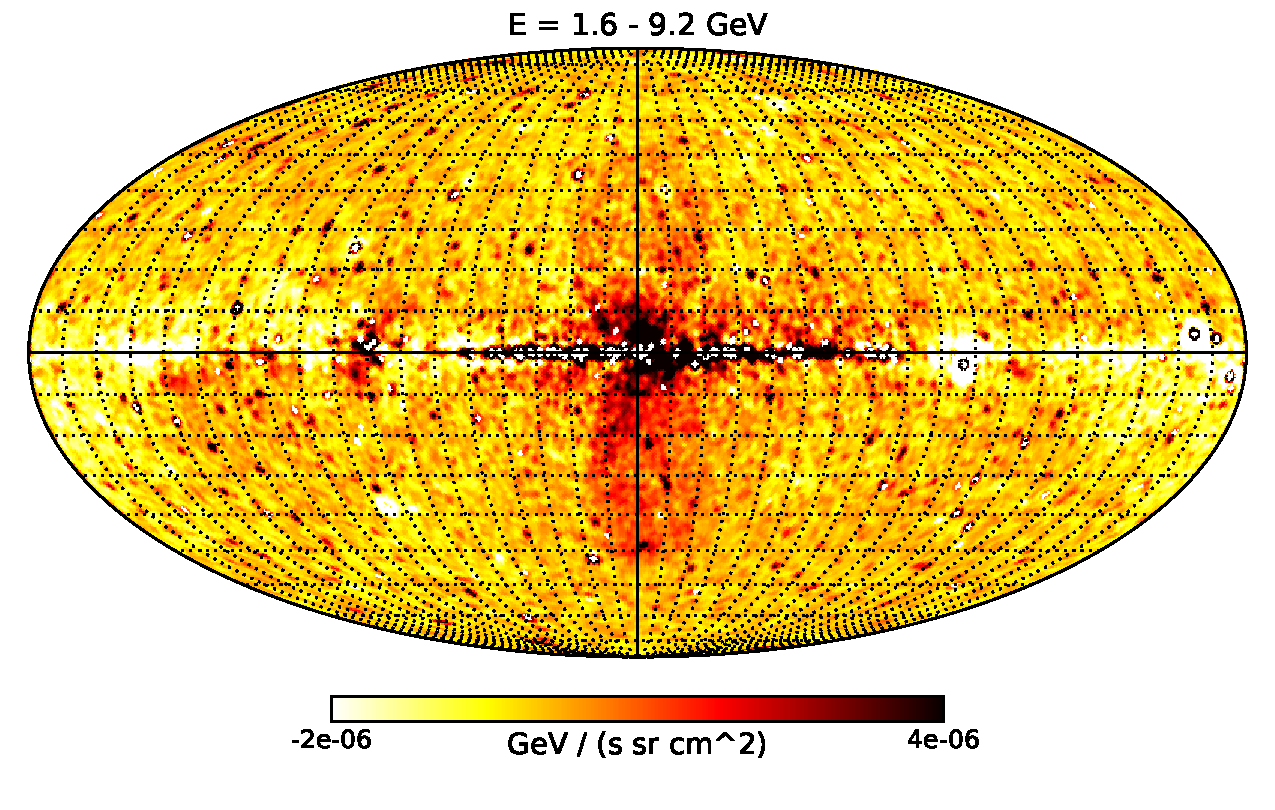
\includegraphics[width=\textwidth]{plots/LowE_06-16GeV_smallmask_bubblesexcl_highEsmooth_symmask_tot_highlow_hot.pdf}
    	\end{subfigure} 
    	\begin{subfigure}{0.3\textwidth}
        	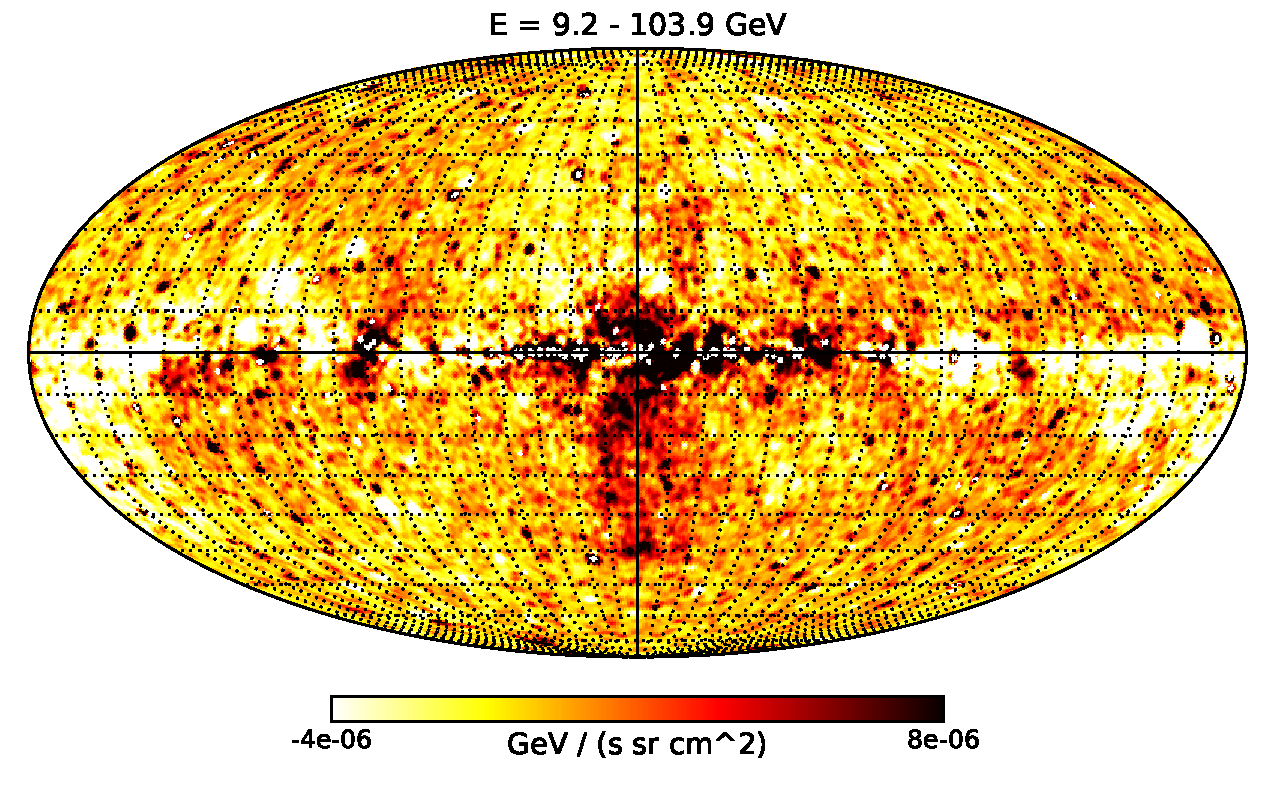
\includegraphics[width=\textwidth]{plots/LowE_06-16GeV_smallmask_bubblesexcl_highEsmooth_symmask_tot_highmedium_hot.pdf}
    	\end{subfigure}
    	\begin{subfigure}{0.3\textwidth}
        	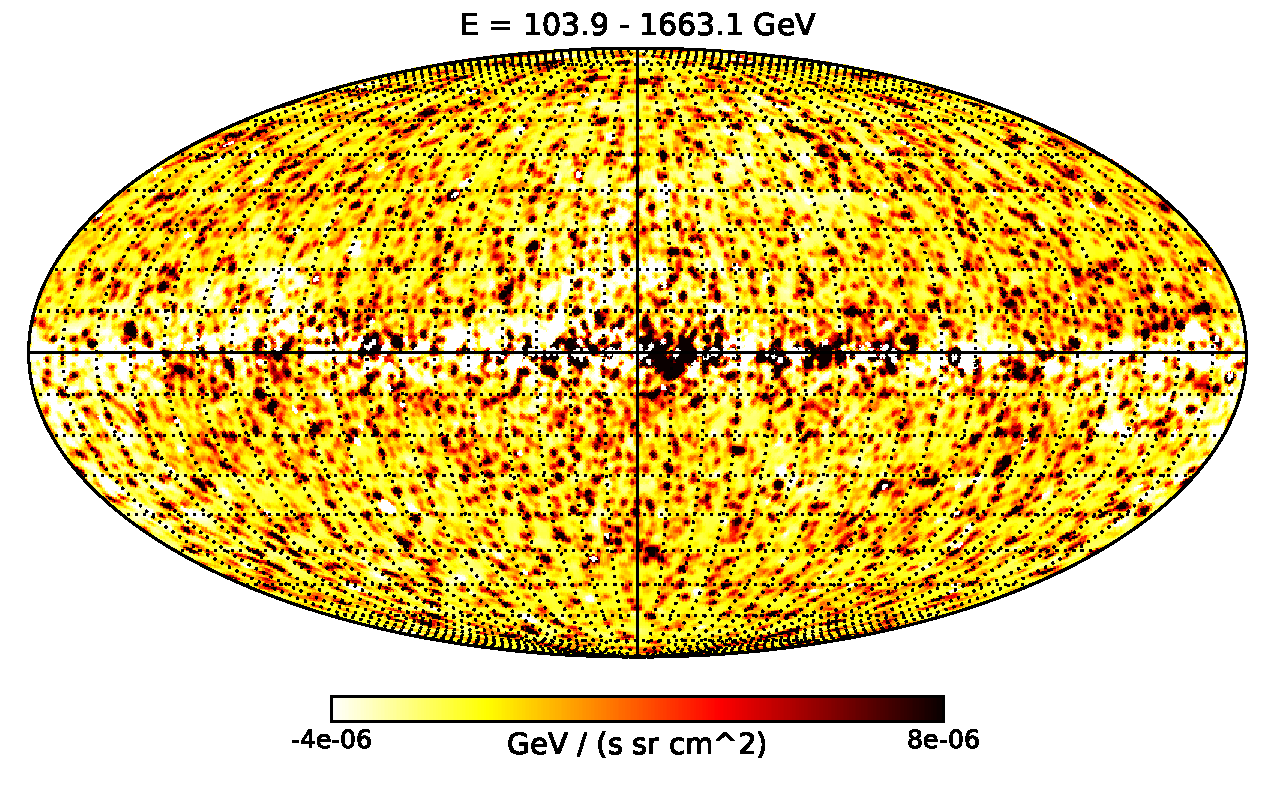
\includegraphics[width=\textwidth]{plots/LowE_06-16GeV_smallmask_bubblesexcl_highEsmooth_symmask_tot_highhigh_hot.pdf}
    	\end{subfigure}
    }
  	\caption{Residuals of the low-energy model for three different energy ranges in differential flux. The \Fermi bubbbles are clearly visible in the first two energy ranges. Point sources are masked.}
  	\label{Maps_lowE}
\end{figure*}

Emission from hadronic interactions dominates in the lower energy range (0.6 - 1.6 GeV). Low-energy \Fermi data is a good tracer for hadronic emission in the Galactic plane and can be used to create a spatial template for the Galactic foreground. \\
We cut the sky horizontally in $4^\circ$-thick latitude stripes and define our model in each stripe and energy bin separately. In the latitude stripe $\ell$ and energy bin $E$ our model consists of a term proportional to the low-energy photon counts $k \cdot N^\low$ (summed over all energies in 0.6 - 1.6 GeV) and an additional constant factor $c$: $N^\model_{\ell E} = k_{\ell E} \cdot N^\low_{\ell E} + c_{\ell E}$. The constant factor $c$ takes into account the isotropic extragalactic background and compensates for the latitude dependent IC emission. We fit the model to the high-energy \Fermi data (with python's iminuit and a likelihood fit) and obtain the fit parameters $c$ and $k$. Since the point spread function is significantly worse for smaller energies, we smoot the high-energy data with a Gaussian prior to the fit. To avoid an overcompensation of the \Fermi bubbles the region $-20^\circ < \ell < 20^\circ$ is excluded from the fit. Certain point sources from the 2FGL catalog are masked \Laura{The mask covers the 200 brightest gamma-ray sources of the 2FGL with a circle of radius $\frac{\delta}{\sqrt{2}} + 1^\circ$ with $\delta$ being the angle spanned by the sidelength of one pixel?}. Since there are many point sources at low latitudes, that could introduce a bias, the mask is symmetrized w.r.t. the Galactic center. \\
Figure \ref{Maps_lowE} shows the resulting residual maps for three different energy ranges. The \Fermi bubbles are clearly visible in the first two energy ranges, $E = 1.6 - 9.2$ GeV and $E = 9.2 - 103.9$ GeV, for $E = 103.9 - 1663.1$ GeV the statistics are too low.  


\subsection{Rectangles model of the bubbles}
First simple ansatz to 

\subsection{GALPROP model of the foreground and PS refitting}


\begin{figure*}
	\makebox[\textwidth][c]{
    	\begin{subfigure}{0.3\textwidth}
        	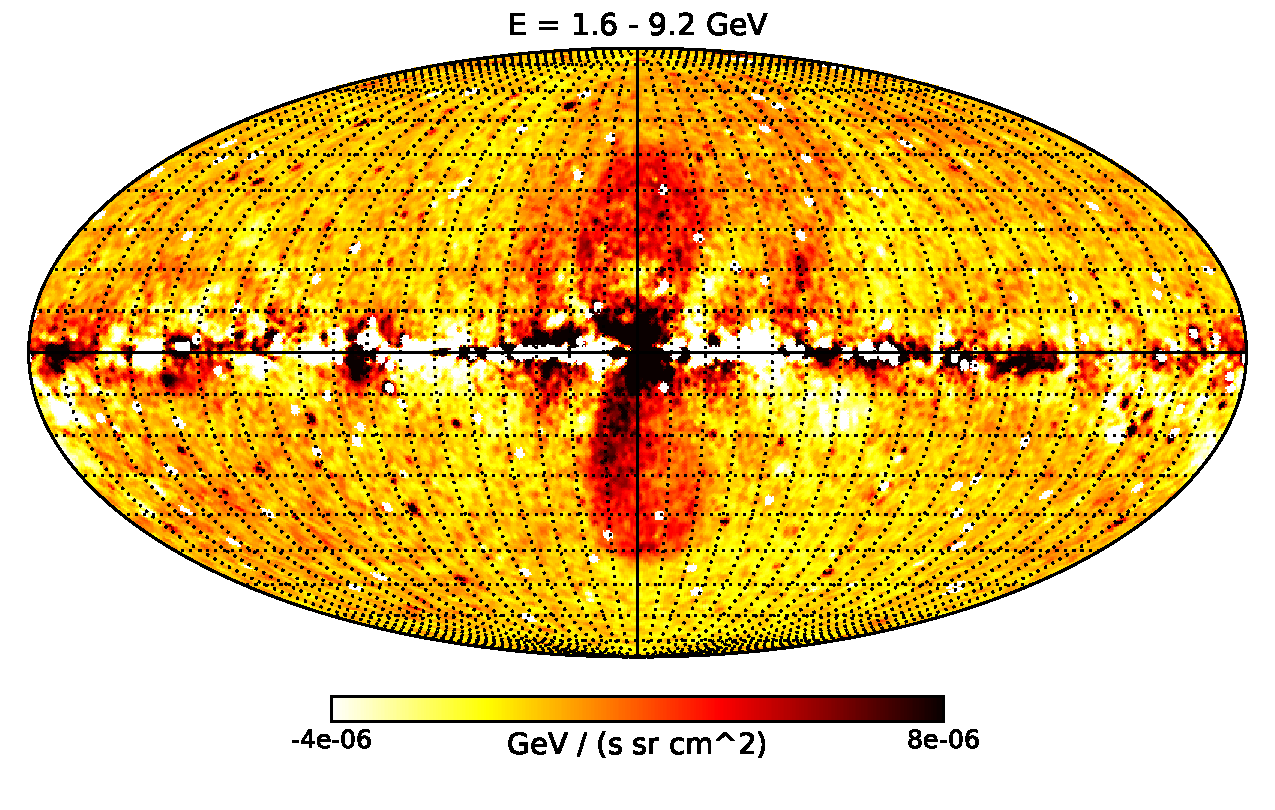
\includegraphics[width=\textwidth]{plots/Source_refit_3FGL_40PS_resid_signal_bubbles_flux_highlowE_hot.pdf}
    	\end{subfigure} 
    	\begin{subfigure}{0.3\textwidth}
        	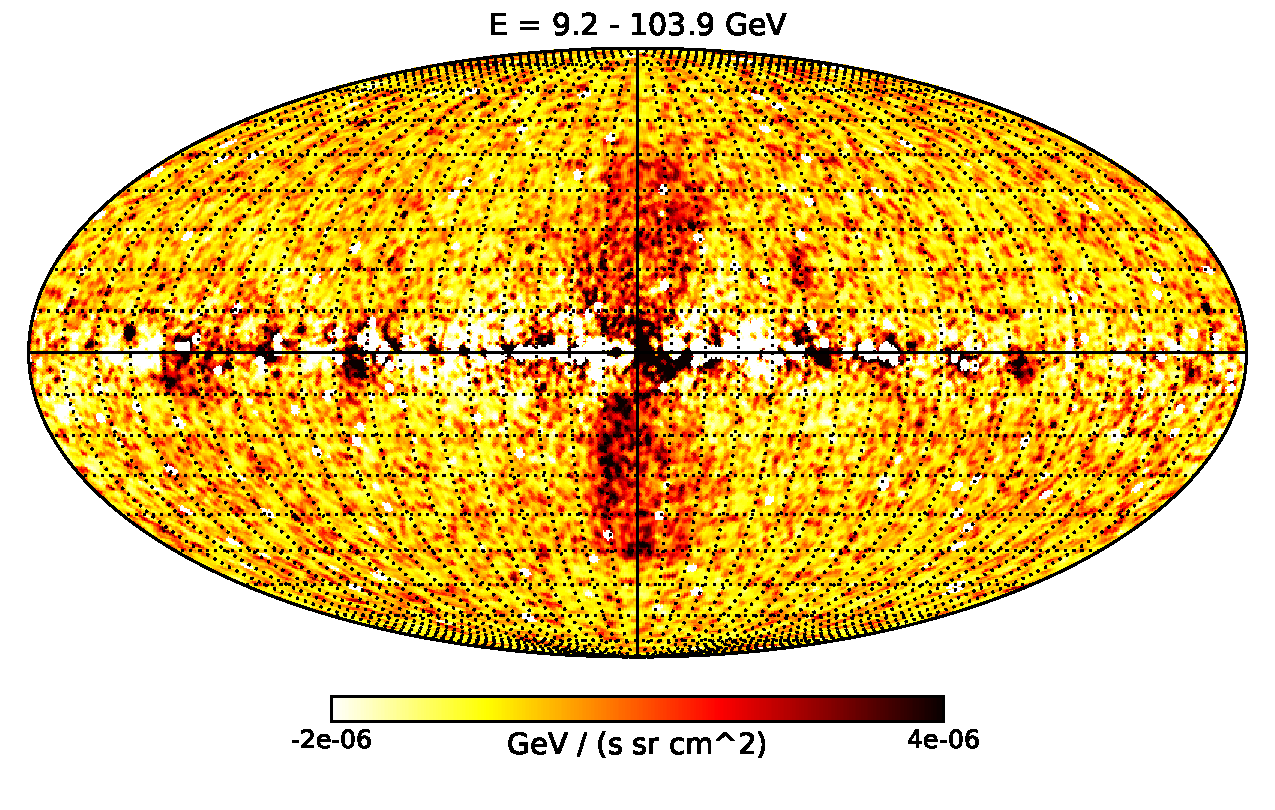
\includegraphics[width=\textwidth]{plots/Source_refit_3FGL_40PS_resid_signal_bubbles_flux_highmediumE_hot.pdf}
    	\end{subfigure}
    	\begin{subfigure}{0.3\textwidth}
        	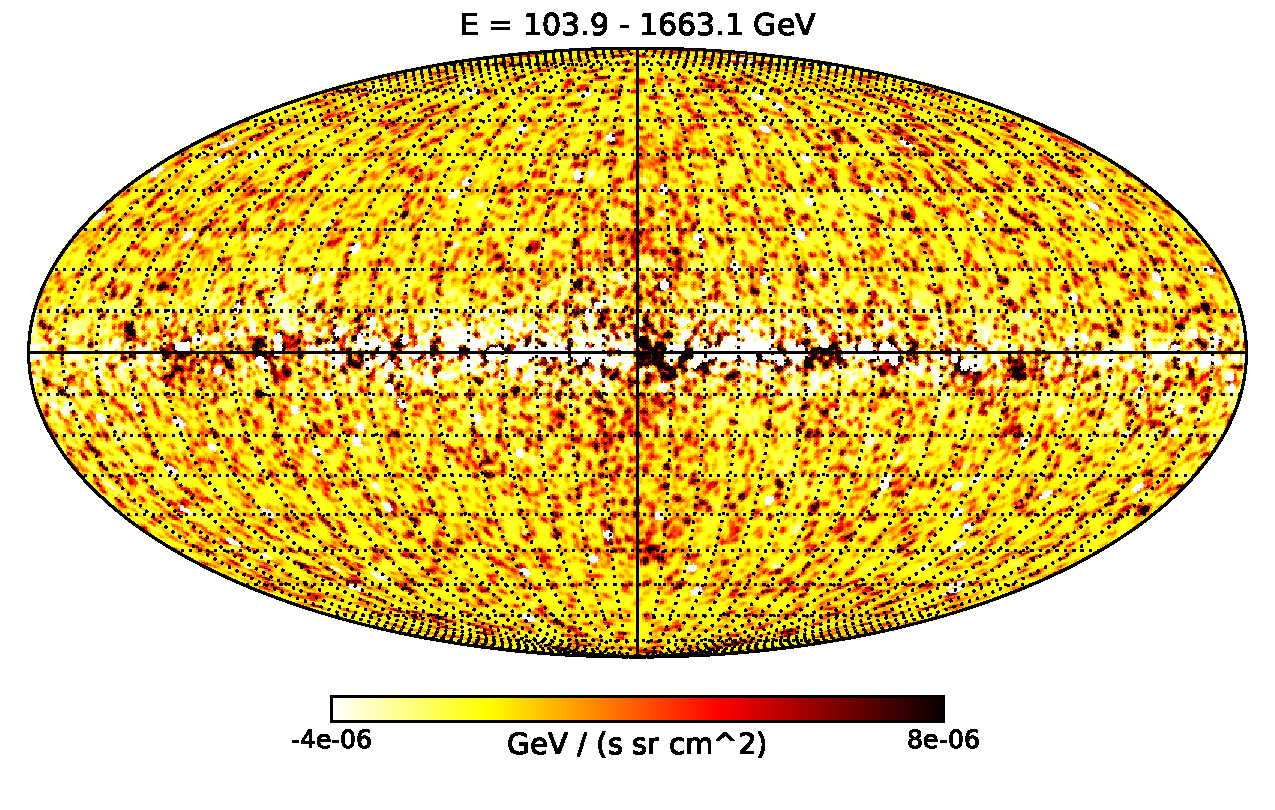
\includegraphics[width=\textwidth]{plots/Source_refit_3FGL_40PS_resid_signal_bubbles_flux_highhighE_hot.pdf}
    	\end{subfigure}
    	}
  	\caption{GALPROP model residuals in three different energy ranges.}
  	\label{Maps_GALPROP}
 \end{figure*}
